\documentclass{beamer}
\usetheme{Wrexham}  
\usepackage{graphicx}
\usepackage{algorithm}
\usepackage{algorithmic}
\usepackage{caption}
\usepackage{subcaption}
\graphicspath{{./figures/}}
\begin{document}
\title{What is Texture?}
%\subtitle{A friendly introduction to compressive sensing.}
\author{Rhian Davies}
\titlegraphic{ 
\includegraphics[height=.2\textheight]{logoEPSRC.png} \hspace{3cm} 
\includegraphics[height=.2\textheight]{logoSTORi.png}}
\date{\today}

\begin{frame}[plain] 
  \titlepage
\end{frame}

\begin{frame}
\begin{figure}[h]
  \centering
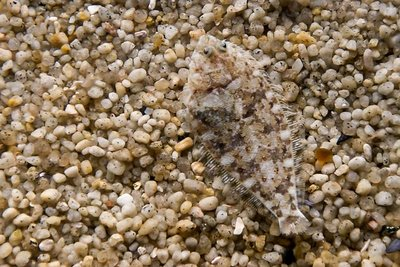
\includegraphics[width = 8cm]{fish}
\end{figure}
\end{frame}

\begin{frame}
\begin{figure}[h]
  \centering
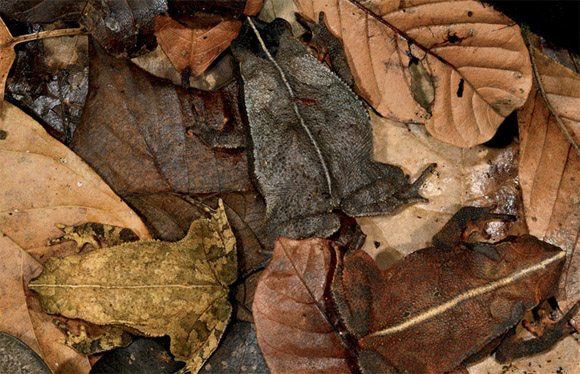
\includegraphics[width = 8cm]{toads}
\end{figure}
\end{frame}

\begin{frame}
  \begin{figure}[h]
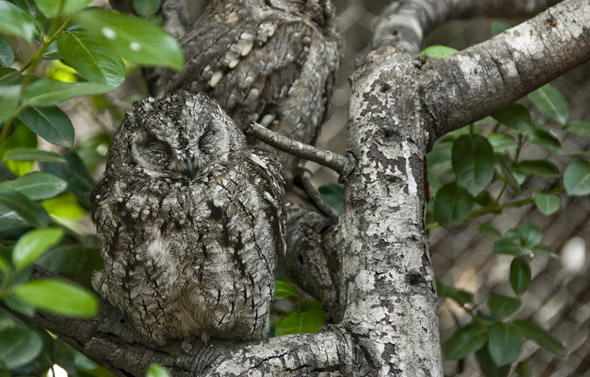
\includegraphics[width = 8cm]{owl}    
  \end{figure}
\end{frame}


\begin{frame}
  \begin{figure}[h]
    \centering
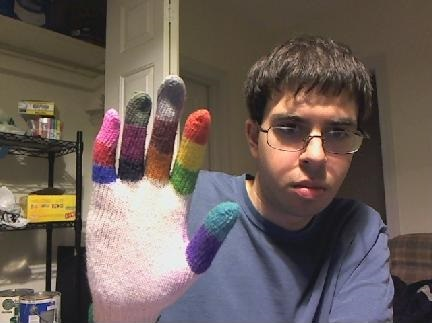
\includegraphics[width = 6cm]{hand}    
  \end{figure}
\end{frame}


\begin{frame}
  \begin{figure}[h]
    \centering
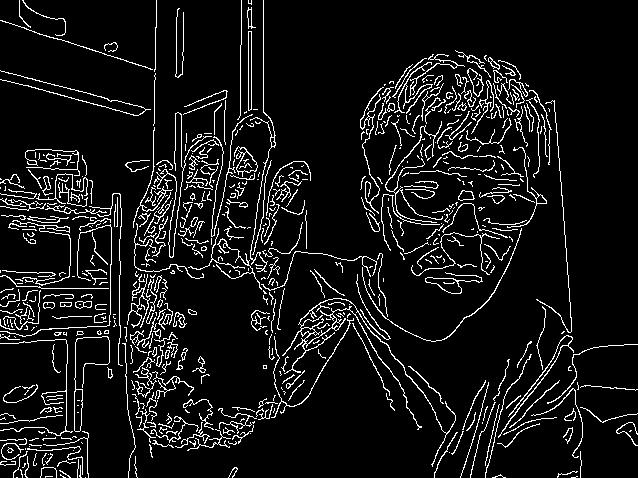
\includegraphics[width = 6cm]{edgeFail}    
  \end{figure}
\end{frame}

\begin{frame}
  \frametitle{What is texture?}

  \begin{figure}[h]
    \centering
    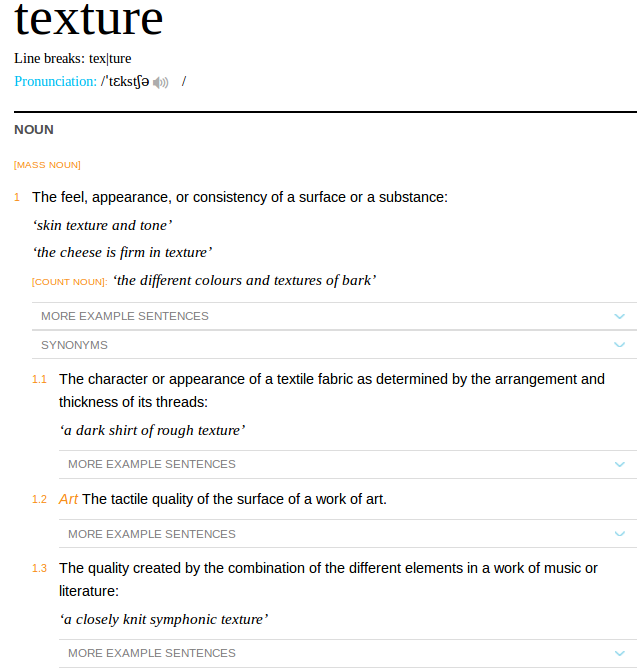
\includegraphics[width = 8cm]{def}
  \end{figure}
 
 \end{frame}


\begin{frame}
\frametitle{Haralick's Thoughts on  Visual Texture}
An innate property of all virtually all surfaces. It contains important information about the structural arrangement of surfaces and their relationship to the  surrounding environment.


Texture can be considered an organised area phenomena. When it is decomposable it has two basic dimensions. The first dimension is for describing primitives out of which the image is composed and the second dimension is for the description of the spatial dependence or interaction between the primitives of an image texture.  

\begin{figure}[h]
  \centering
  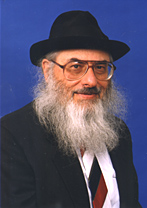
\includegraphics[width = 3cm]{haralick_robert}
\end{figure}

\end{frame}

\begin{frame}
\frametitle{Primitive?}
 

  \begin{itemize}
  \item Collection of pixels which form a basic element of a textured image
    \item Scale dependency is required for texture description.  
  \end{itemize}

\begin{figure}[h]
        \centering
        \begin{subfigure}[b]{0.4\textwidth}
          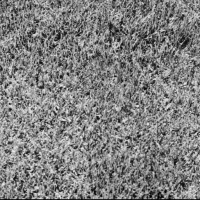
\includegraphics[width=\textwidth]{grass}
                \caption{Grass}
                \label{fig:ma}
        \end{subfigure}
        ~ %add desired spacing between images, e. g. ~, \quad, \qquad etc.
          %(or a blank line to force the subfigure onto a new line)
        \begin{subfigure}[b]{0.4\textwidth}
                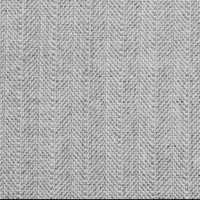
\includegraphics[width=\textwidth]{herringbone}
                \caption{Herringbone}
                \label{fig:mm}
        \end{subfigure}
   %     \caption{Output clusters for test image D}\label{Herringbone}
\end{figure}

\end{frame}

\begin{frame}
  \begin{figure}[h]
    \centering
    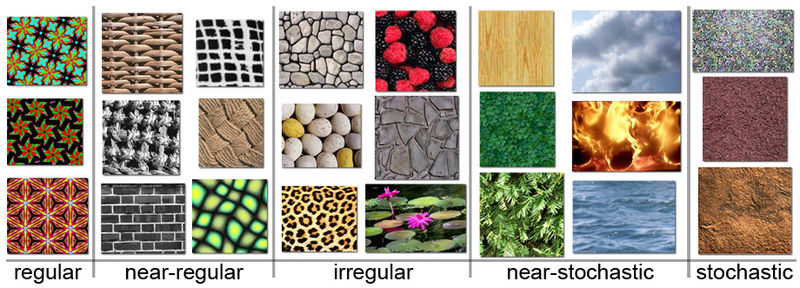
\includegraphics[width = 10cm]{stoc}
  \end{figure}

\end{frame}

\begin{frame}
  
\begin{figure}[!ht]
  \centering
  \subfloat{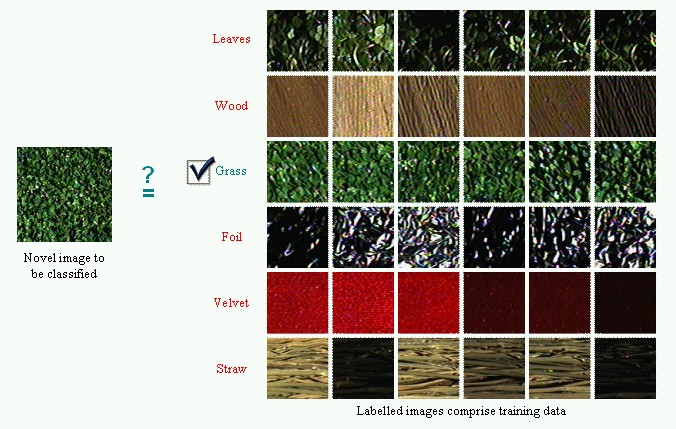
\includegraphics[height = 3cm]{im2}}\quad \quad \quad \quad
  \subfloat{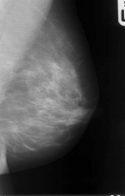
\includegraphics[height = 3cm]{im1}}\\  
\hspace{1cm}\\
  \subfloat{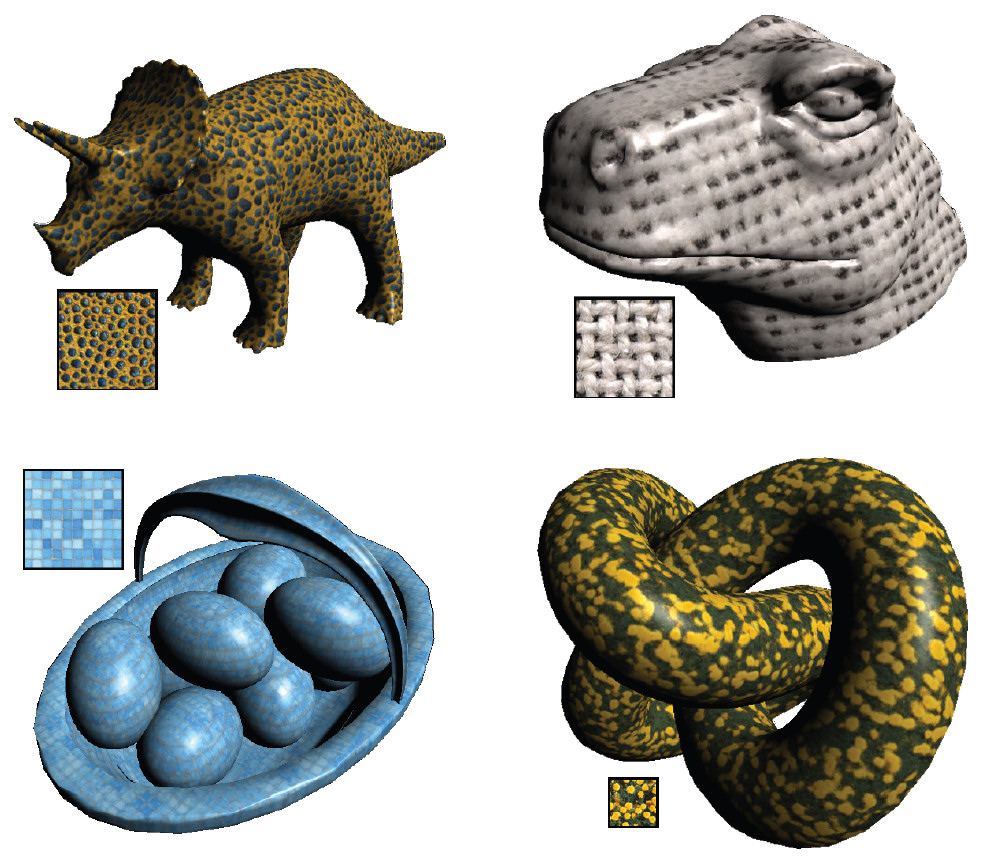
\includegraphics[height = 3cm]{im5}}\quad \quad \quad \quad \quad \quad \quad \quad
  \subfloat{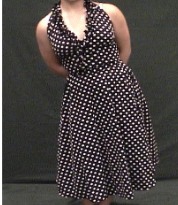
\includegraphics[height = 3cm]{im4}}
 % \caption{First group of subfigures.}
 % \label{fig:sub1}
\end{figure}
\end{frame}


\begin{frame}
  \frametitle{Texture Segmentation}
  \begin{itemize}
 \item Challenge: Partition image into disjoint regions of a coherent texture. 
\item We don't know...
\item What types of textures exist in an image
\item How many different textures there are
 
\item Approach is to generate texture features to describe and then cluster. 

  \end{itemize}
  \begin{figure}[h]
    \centering
    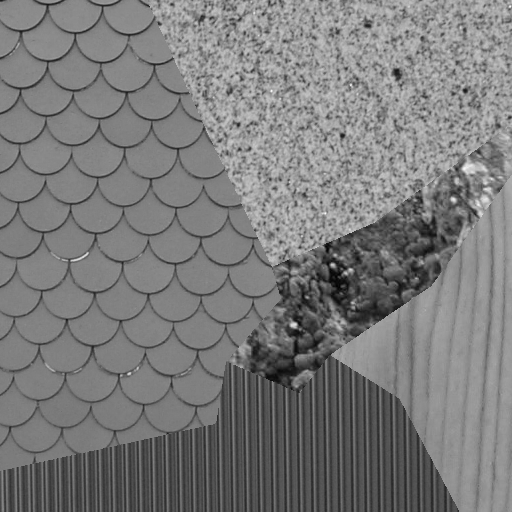
\includegraphics[width = 4cm]{tm3_1_1}
  \end{figure}

\end{frame}



\begin{frame}
  \frametitle{Texture Feature Extraction}

  \begin{itemize}
  \item Auto correlation Function $\frac{\frac{1}{(N_i - |x|)(N_j - |y|)}\sum_{i}\sum_{j}I(i,j)I(i+x,j+y)}{\frac{1}{N_iN_j}\sum_{i=1}^{N_i}\sum_{j=1}^{N_j}I(i,j)^2}$
\item Co-occurrence Matrix
\item Wavelet Transform 
  \end{itemize}

\begin{figure}[h]
        \centering
        \begin{subfigure}[b]{0.32\textwidth}
          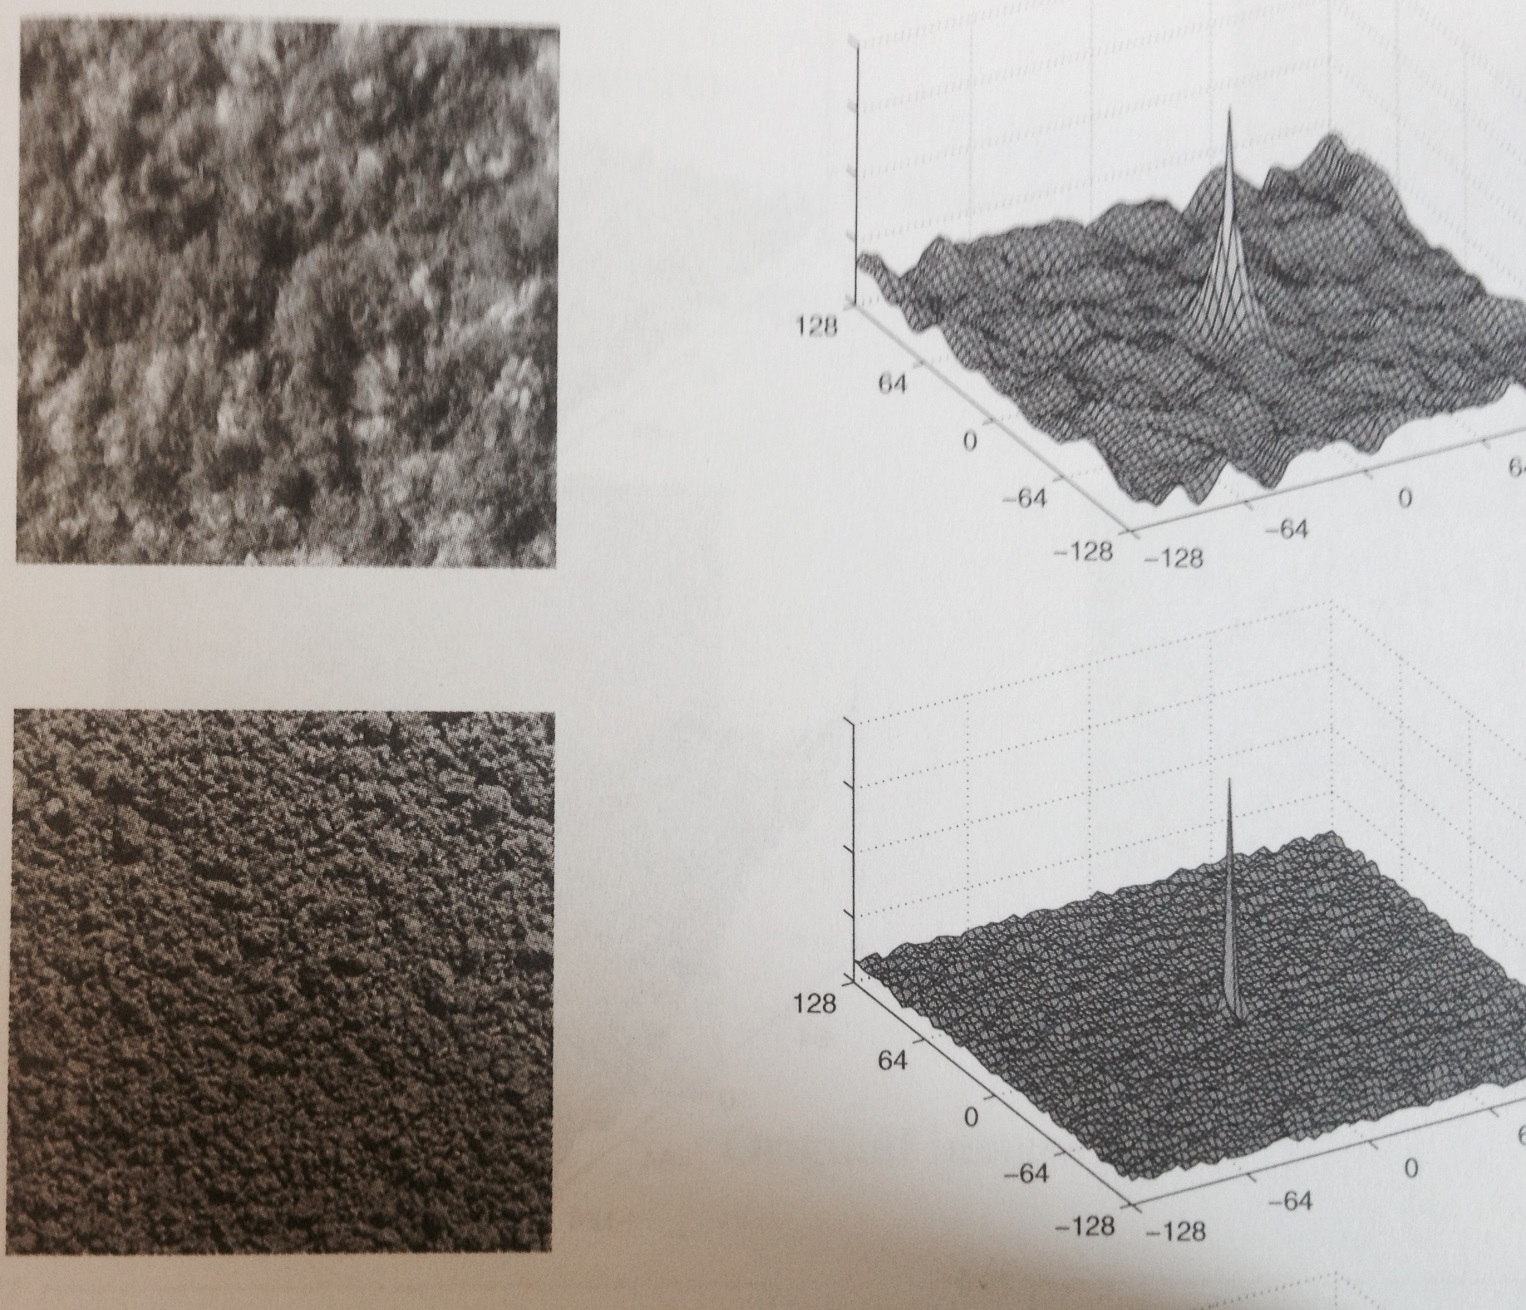
\includegraphics[width=3cm]{acf2}
        \end{subfigure}
               \begin{subfigure}[b]{0.32\textwidth}
                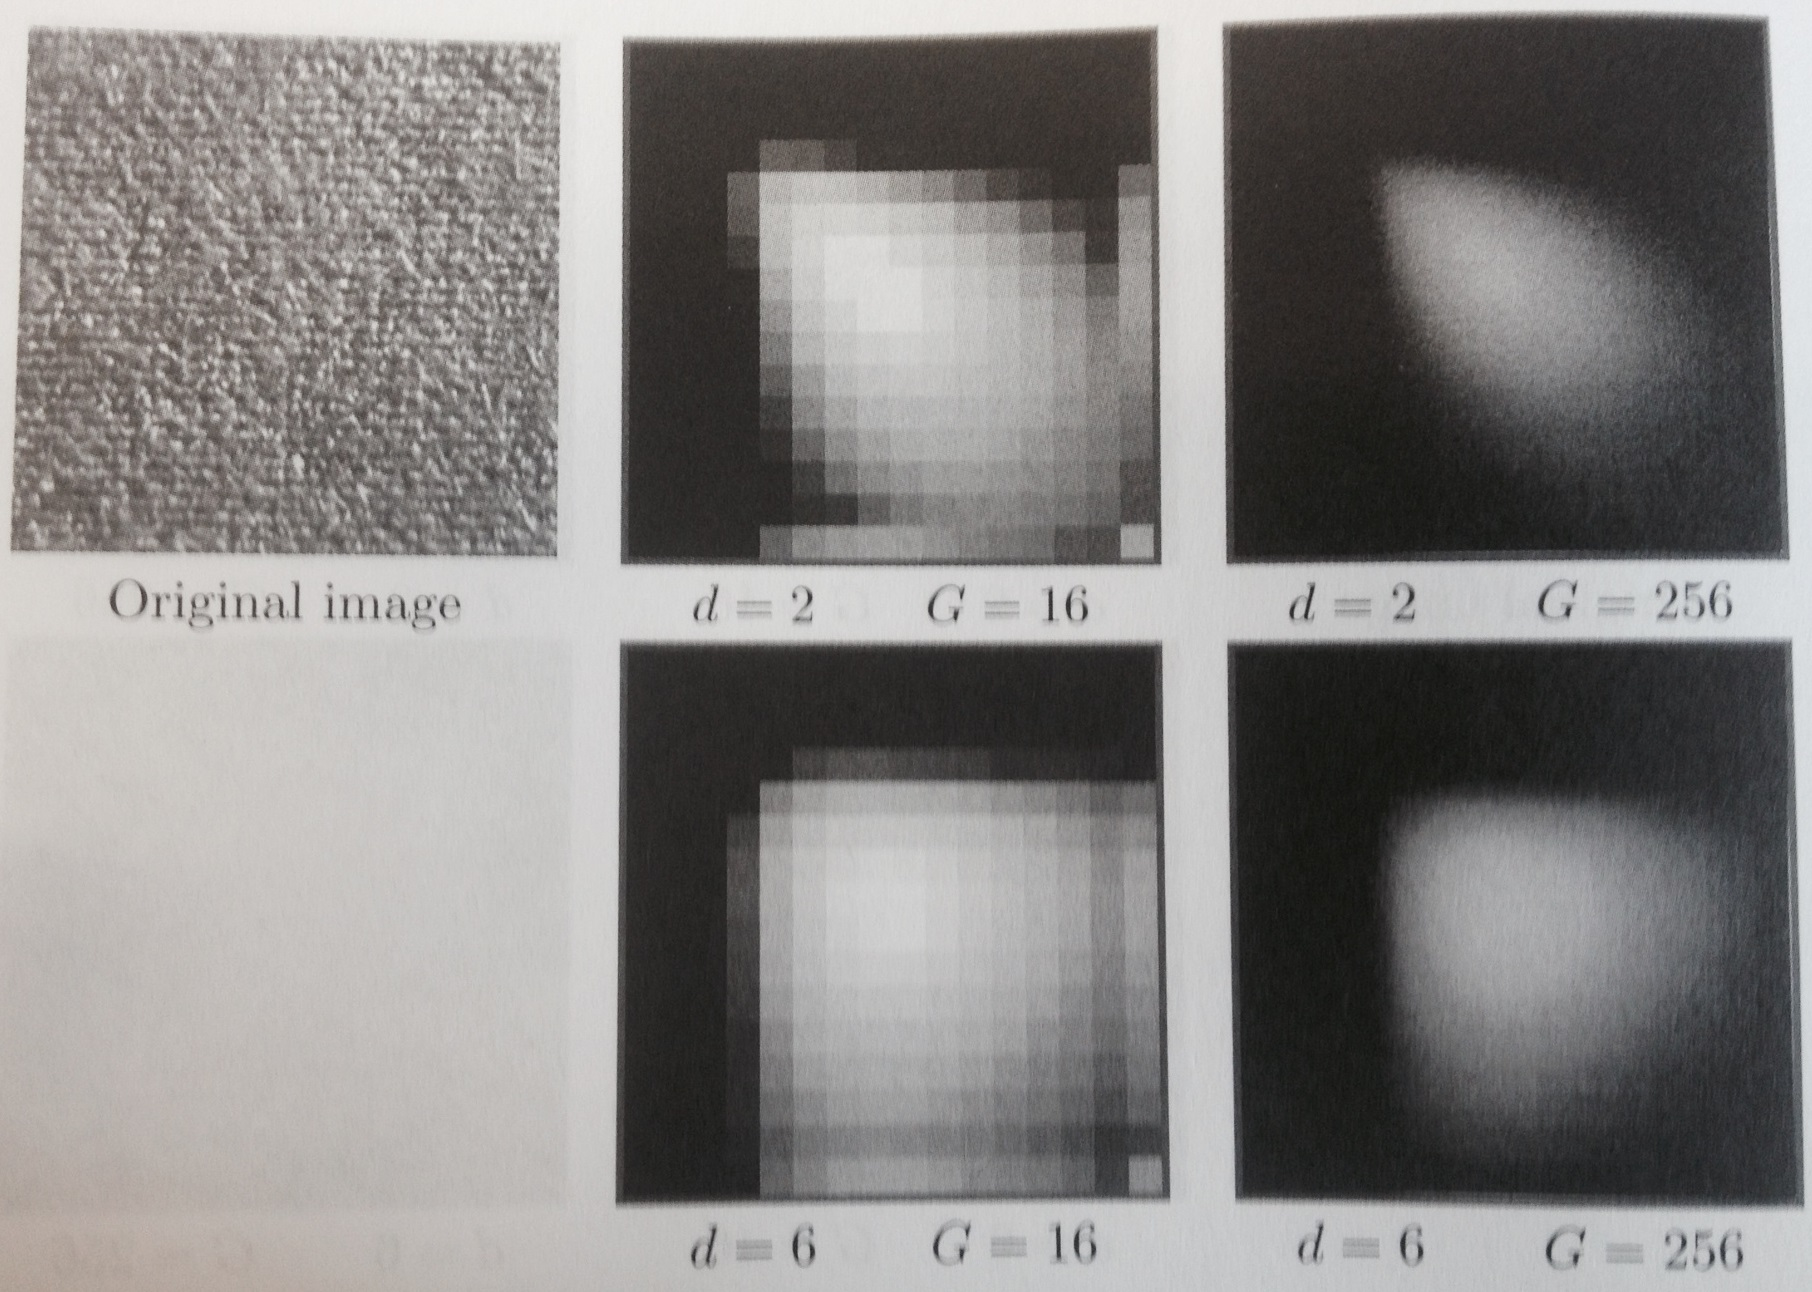
\includegraphics[width=3cm]{coocc}
        \end{subfigure}
  \begin{subfigure}[b]{0.32\textwidth}
                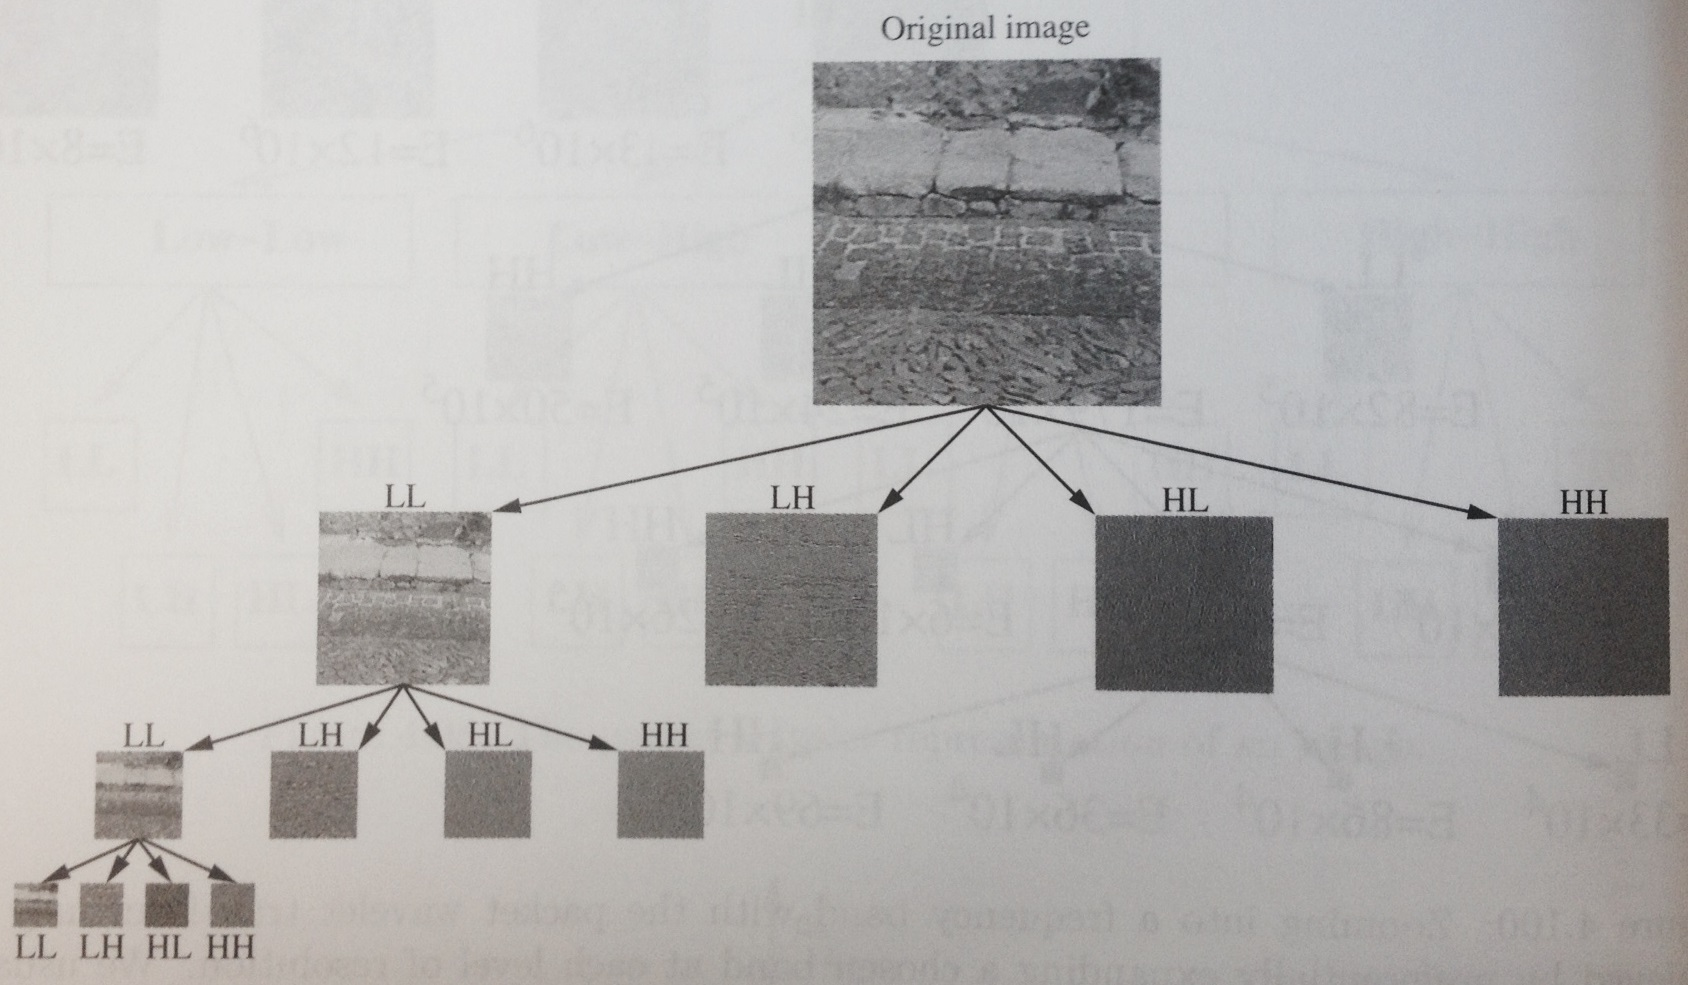
\includegraphics[width=3cm]{wavtree}
        \end{subfigure}
 \end{figure}

\end{frame}








\begin{frame}
  \begin{figure}[h]
    \centering
    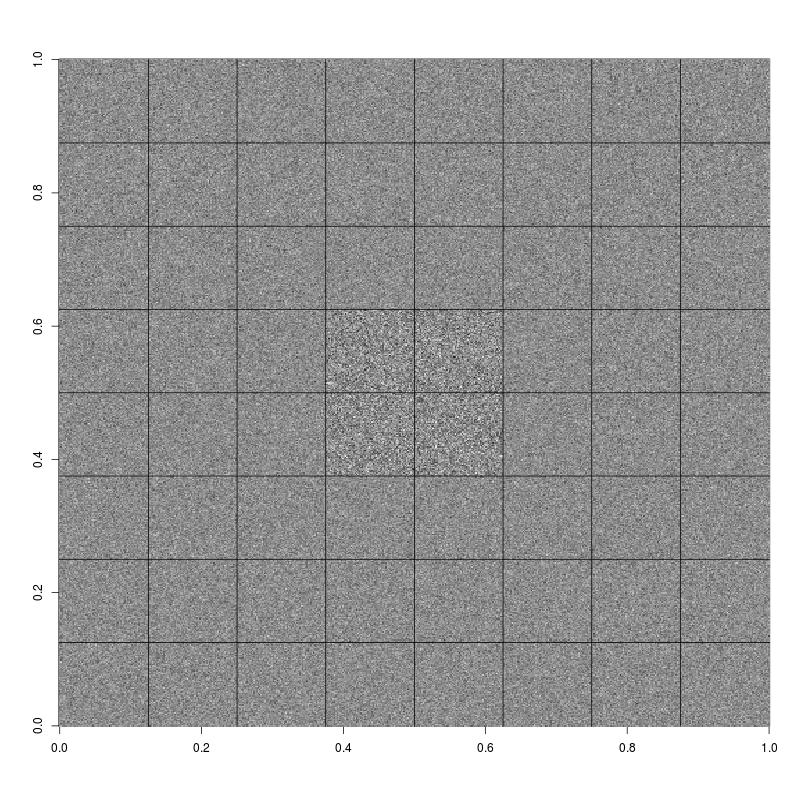
\includegraphics[width = 6cm]{test_64_}
  \end{figure}
\end{frame}


\begin{frame}
  
\begin{figure}[h]
  \centering
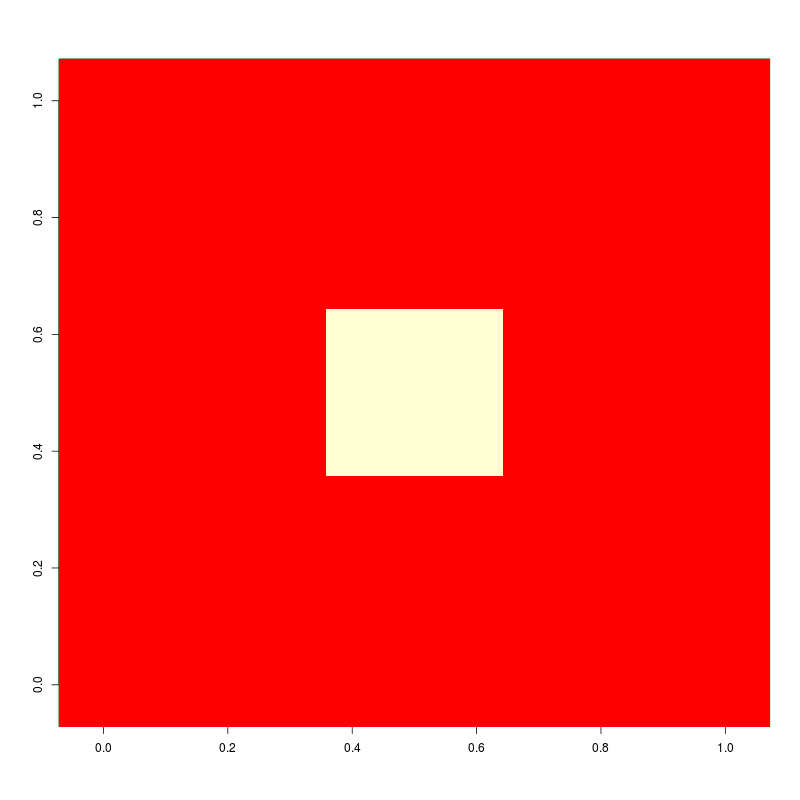
\includegraphics[width=6cm]{cluster_2_64_}
\end{figure}
\end{frame}

\begin{frame}
  
\begin{figure}[h]
  \centering
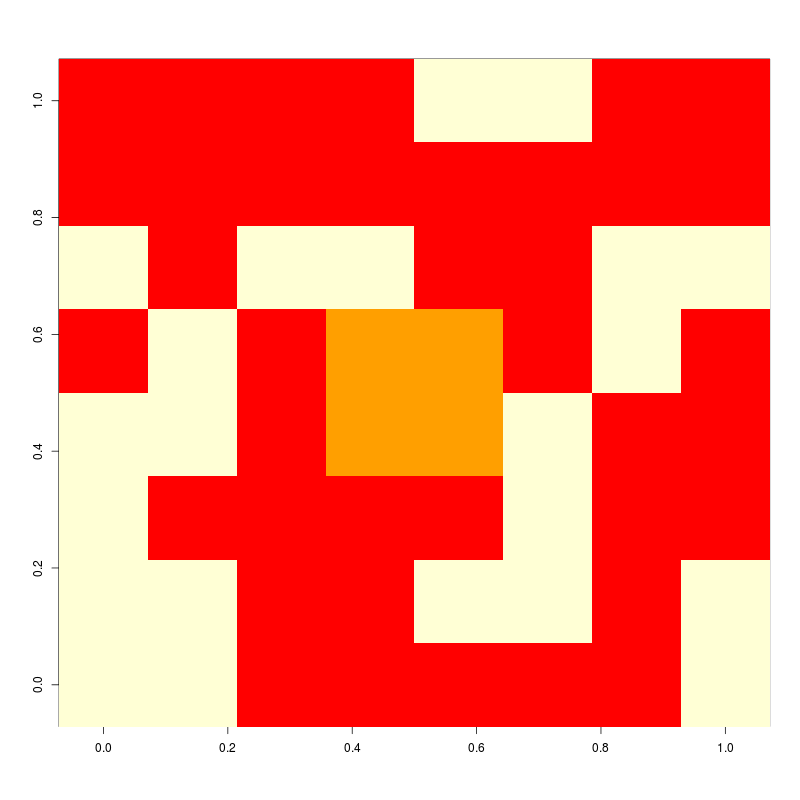
\includegraphics[width=6cm]{cluster_3_64_}
\end{figure}
\end{frame}








 \end{document}


\begin{frame}
 \frametitle{Statistical generation of texture features.}

Statistical methods analyse the spatial distribution of gray values, by computing local features at each point in the image, and deriving a set of statistics
from the distributions of the local features. 

Depending on the number of pixels defining the local feature, statistical methods can be further classified into first-order (one pixel), second-order (t
wo pixels) and higher-order (three or more pixels) statistics.  First-order statistics estimate properties (e.g. average and variance) of individual pixel values, ignoring the spatial interaction between image pixels, whereas second- and higher-order statistics estimate properties of two or more pixel values occurring at specific locations relative to each other. 

\end{frame}


\begin{frame}
  \frametitle{Spectral Approaches}
  \begin{itemize}
  \item Texture description is highly scale dependant.
    \item Decrease the scale sensitivity, describe texture in multiple resolutions and an appropriate scale may be chosen to achieve the maximum texture discrimination. 
\item Fourier and wavelet transforms common choices

Wavelet transforms feature several advantages  over gabor transform for segmentation. 
 Varying the spatial resolution allows it to rep\begin{frame}
  \frametitle{What's next?}

  \begin{itemize}
\item New feature extraction methods for 
\item C
  \item What to do with the borders?
    \item Illumination issues. 
\item Adaptive feature matrix generation?
  \end{itemize}



\end{frame}
resent textures at the most suitable scale,
There is a wide range of choices for the wavelet function, so one is able to choose wavelets best suited for texture analysis in a specific application.
  \end{itemize}

\begin{frame}
  \frametitle{What's next?}

  \begin{itemize}
\item New feature extraction methods for 
\item C
  \item What to do with the borders?
    \item Illumination issues. 
\item Adaptive feature matrix generation?
  \end{itemize}



\end{frame}






\end{frame}



\begin{frame}
 There are 3 principal statistical approaches used in image processing to describe the texture of a region:
 Basic or First Order
 Structural or Second Order
Spectral approaches.

The Basic Statistical approaches yield characterizations of textures as smooth, coarse, grainy, and so on.
 One of the simplest approaches for describing texture is to use moments of the gray-level histogram of an image or region.

Structural approaches deal with the arrangement of image primitives. They use a set of predefined texture primitives and a set of construction rules to
define how a texture region is constructed with the primitives and the rules.

Spectral approaches to texture analysis techniques are based on properties of the Fourier spectrum, Gabor and wavelet based and are used primarily to detect global periodicity in an image by identifying high energy, narrow peaks in the spectrum. 
\end{frame}


\begin{frame}
  
\begin{figure}[h]
  \centering
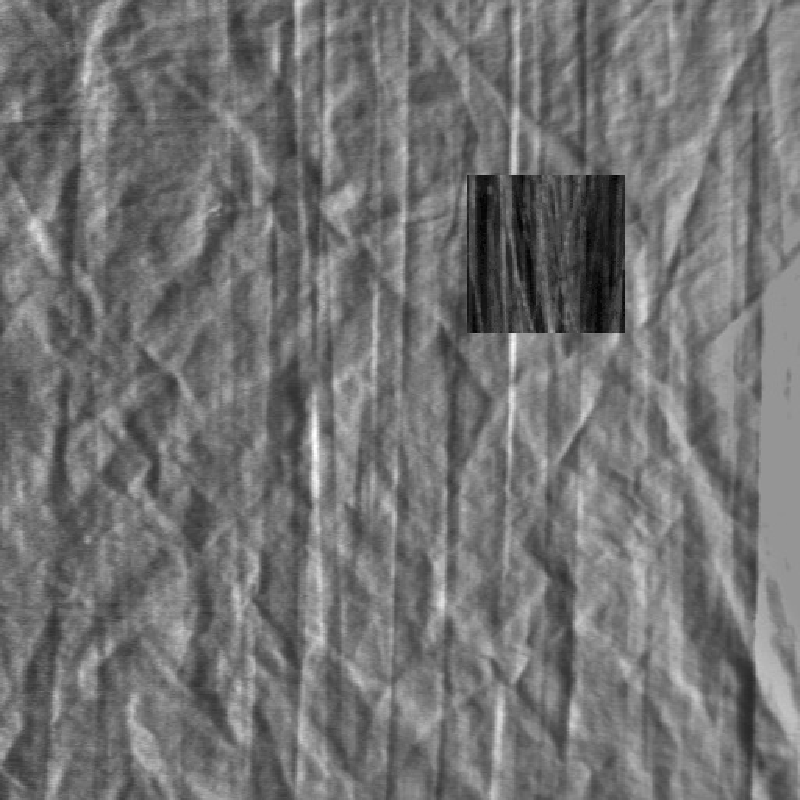
\includegraphics[width=6cm]{testImage_D}
\end{figure}
\end{frame}

\begin{frame}
  
\begin{figure}[h]
  \centering
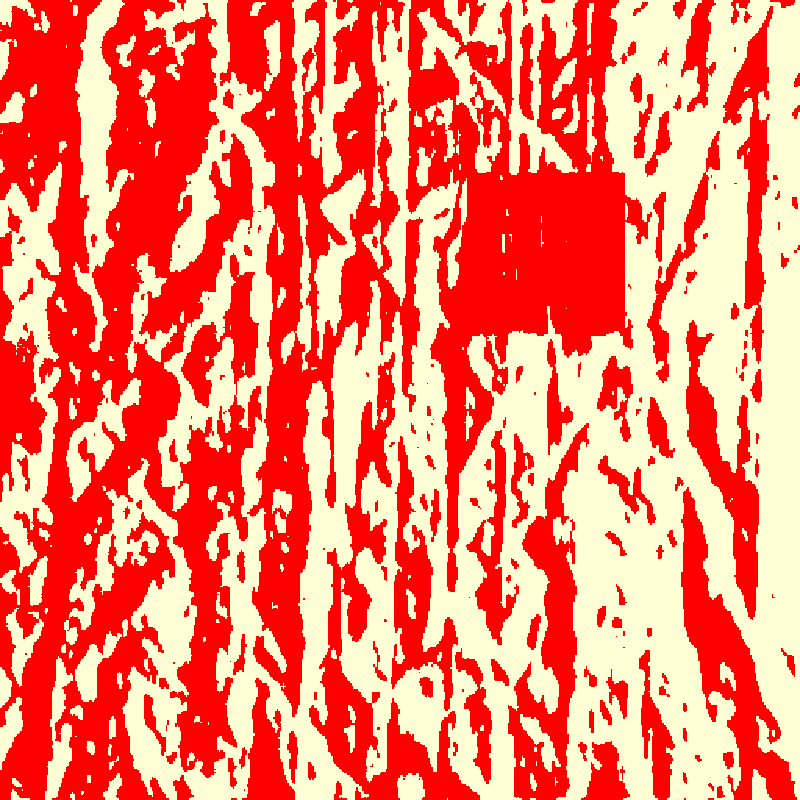
\includegraphics[width=6cm]{kmeans2_d_ma}
\end{figure}
\end{frame}